\documentclass[12pt]{article}
\usepackage[utf8]{inputenc}
\usepackage{lmodern}
\usepackage[T1]{fontenc}
\usepackage{amsmath}
\usepackage{enumitem}
\usepackage{graphicx}
\usepackage{fullpage}
\usepackage{siunitx}
\usepackage{fancyhdr}
\PassOptionsToPackage{hyphens}{url}
\usepackage[hyphens]{url}
\usepackage{color}
\usepackage{enumitem}
\usepackage{textcomp}
\usepackage{geometry}
\usepackage{courier}
\usepackage{listings}
\usepackage{array}
\usepackage{amsthm}
\usepackage{mathdots}
\usepackage{amssymb}
\usepackage{minted}
\usepackage{wrapfig}
\usepackage{titlesec}
\usepackage{parskip}
\usepackage{accents}
\usepackage{gensymb}
\usepackage{indentfirst}
\usepackage{courier}
\usepackage{framed}
\usepackage{etoolbox}
\usepackage{titlesec}
\usepackage{appendix}
\usepackage{mdframed}
\usepackage{verbatim}
\usepackage{xspace}
\usepackage{hyperref}
\AtBeginEnvironment{subappendices}{%
	\section*{Appendix}
	\addcontentsline{toc}{section}{Appendices}
}

%\lstset{language=C++,
%                basicstyle=\ttfamily,
%                keywordstyle=\color{blue}\ttfamily,
%                stringstyle=\color{red}\ttfamily,
%                commentstyle=\color{green}\ttfamily,
%                morecomment=[l][\color{magenta}]{\#}
%}

\definecolor{keywordcolor}{rgb}{0,0,0.45}
\definecolor{stringcolor}{rgb}{0.45,0.45,0.45}
\definecolor{commentcolor}{rgb}{0,0.3,0}

\lstset{
	language=C++,
	basicstyle=\footnotesize\ttfamily,
	numbers=left,
	%numberstyle=\tiny,
	frame=tb,
	columns=fullflexible,
	showstringspaces=false,
	breaklines=true,
	tabsize=4,
	keywordstyle=\color{keywordcolor}\footnotesize\bf\ttfamily,
	stringstyle=\color{stringcolor}\footnotesize\ttfamily,
	commentstyle=\color{commentcolor}\it\sffamily
}
% \lstset{basicstyle=\ttfamily,breaklines=true}
\lstloadlanguages{C++}

%\renewcommand{\familydefault}{\sfdefault}

\addtolength{\parskip}{\baselineskip}  
\newcommand{\urlwofont}[1]{\urlstyle{same}\url{#1}}

\renewcommand{\arraystretch}{0.8}
\renewcommand{\headrulewidth}{0pt}
\renewcommand{\footrulewidth}{0pt}

\newcommand{\imagewidth}{0.8\textwidth}

\lhead{}
\chead{}
\rhead{}
\lfoot{}
\cfoot{\thepage}
\rfoot{}

\geometry{
	top=0.9in,
	inner=0.7in,
	outer=0.7in,
	bottom=0.9in,
	headheight=2ex,
	headsep=1ex,
}
\pagestyle{fancy}
%\fancyhf{}
%\setlength{\headsep}{0.2in}


\fancypagestyle{firststyle}
{
	\chead{}
	\setlength{\headsep}{0.0in}
}
\hypersetup{
	unicode=true,
	colorlinks=true,
	linkcolor=blue,
	citecolor=black,
	filecolor=black,
	urlcolor=blue
}

\begingroup
\makeatletter
\@for\theoremstyle:=definition,remark,plain\do{%
	\expandafter\g@addto@macro\csname th@\theoremstyle\endcsname{%
		\addtolength\thm@preskip\parskip
	}%
}
\endgroup

\newtheorem{thm}{Theorem}[section]
\newtheorem{lemma}{Lemma}[section]
\newtheorem{claim}{Claim}[section]
\newtheorem{proposition}{Proposition}[section]
%\theoremstyle{empty}
\newtheorem*{namedthm}{Theorem}

% indention size
%\setlength{\parindent}{19pt}
\setlength{\parindent}{0pt}

% paragraph spacing
\setlength{\parskip}{1em}

% line spacing
\linespread{1}

%\setcounter{tocdepth}{1}


% Documenting starts here! Please do not change above! 

\newcommand{\mytitle}
{
	\textbf {
		inzva Algorithm Programme 2018-2019\\ \ \\
		Bundle 11 \\ \ \\ 
		Graph - 3\\ \ \\
	}
}

\title{\vspace{-2em}\mytitle\vspace{-0.3em}}

\author{
	\textbf{Editor}\\
	Ekrem BAL  \\ \ \\ 
	\textbf{Reviewers} \\ 
	Bahadır ALTUN \\
	Yasin KAYA \\
	Burak BUĞRUL \\
}

\date{}
\begin{document}
	
	\begin{figure}
		\centering
		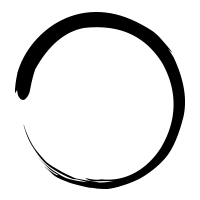
\includegraphics[width=\linewidth/4]{inzva-logo.png}
		\label{fig:inzva}
	\end{figure}
	\maketitle
	
	\cleardoublepage
	\tableofcontents
	\markboth{Table of Contents}{}
	\cleardoublepage
	
	 
    \section{Bridges and Articulation Points}
    \subsection{DFS order}
    \textbf{Dfs order} verilen bir çizgeyi root düğümünü sabitleyerek dfs algoritmasındaki ile aynı şekilde fakat keşfedilmiş bir düğüme bir daha gitmeyerek tüm düğümleri gezmektir. Burada önemli bir gözlem ise kullandığımız kenarlar ve düğümler bir \textbf{tree} yapısı oluşturacaktır. Çünkü her düğüme(\textbf{root hariç}) yalnızca başka bir düğümden geldiğimiz için ve \textbf{root} düğümüne ise herhangi başka bir düğümden gelmediğimizden bu yapı bir \textbf{tree} yapısı oluşturur.
   \begin{minted}[frame=lines,linenos,fontsize=\footnotesize]{c++}
 void dfs(int node){
	used[node] = true;
	for(auto it : g[node])
		if(!used[it])
			dfs(it);
}
   \end{minted}
    
    \subsection{Edge Çeşitleri}
    Bir çizgeyi dfs order ile gezerken görülebilecek birkaç tane kenar tipi vardır. Bu kenarlar bazı çizge algoritmalarını anlamamızda bize çok faydalı olacaktır.
    
    \textbf{Edge çeşitleri:}
\begin{itemize}
	\item \textbf{Tree edge} : Bu kenarlar çizgeyi gezerken kullandığımız ana kenarlardır.
	\item \textbf{Forward edge} : Bu kenarlar daha önce gittiğimiz ve kendi alt ağacımızda bulunan bir düğüme giden kenarlardır.
	\item \textbf{Back edge} : Bu kenarlar daha önce uğradığımız ama dfs işlemini tamamlamamış düğümlere giden kenarlardır.
	\item \textbf{Cross edge} : Bu kenarlar daha önce uğradığımız ve dfs işlemini tamamlamış düğümlere giden kenarlardır.
\end{itemize}

Bu kenarlar için önemli bir gözlem ise çift-yönlü bir çizgede \textbf{cross edge} olmasının imkansız olduğudur. Çünkü dfs işlemini tamamlamış bir düğümden çıkan bir kenarın gezilmemesi olanaksızdır.

\begin{figure}[H]
\centering
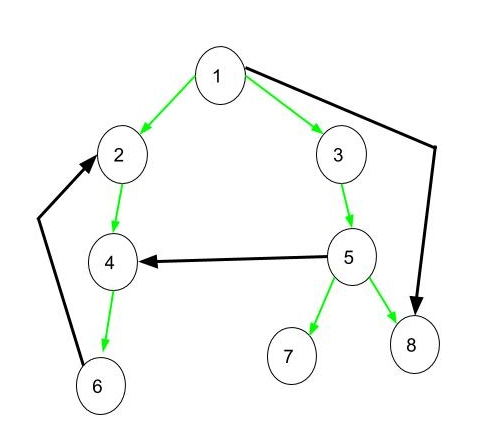
\includegraphics[width=\linewidth/4*2]{edge-cesitleri.png}
\caption{Yeşil renkli kenarler \textbf{tree edge}. (1,8) \textbf{forward edge}. (6,4) \textbf{back edge}. (5,4) \textbf{cross edge}.}
\label{fig:prime1}
\end{figure}

    \subsection{Bridge}
    Yönsüz ve connected bir çizgede eğer bir kenar çıkardığımızda o çizge connected olmaktan çıkıyorsa bu kenara \textbf{bridge} denmektedir.

    \subsection{Bridge Bulma}

    Bridge bulmak için birden fazla algoritma olmasına rağmen (Chain decomposition gibi) aralarında en kolay yazılabilen ve hızlı olan Tarjan'ın algoritmasını ele alacağız.
    
    Bir çizgeyi dfs ile gezerken eğer bir kenarın aşağıdaki ucunun alt ağacından yukarı çıkan bir \textbf{back edge} var ise, o kenar \textbf{bridge} değildir. Çünkü  \textbf{back edge}, bu kenarı çıkardığımızda çizgenin alt ağacının ve atalarının ayrılmasını engellemektedir.

    Bu algoritma da tam olarak buna dayanarak her düğüm için o düğümün alt ağacındaki \textbf{back edge}lerin gittiği minimum derinliği tutmaktadır. 
    
    Eğer bir kenarın alt ucunun alt ağacındaki \textbf{back edge}lerin gittiği minimum derinlik kenarın üst ucunun derinliğinden büyük veya eşitse bu kenar \textbf{bridge}dir. Çünkü bu kenarın alt ucunun alt ağacındaki hiçbir \textbf{back edge}, şuanki kenarımızın üstünde bir düğüme çıkmamaktadır. Dolayısıyla bu kenarı çıkardığımızda çizgenin alt ağacı ve ataları birbirinden ayrılır.
    
    Tarjanın algoritmasıyla çizgedeki bridge'leri O(V + E) zaman karmaşıklığında bulabiliriz. Burada V çizgedeki düğüm sayısını, E ise çizgedeki kenar sayısını temsil etmektedir.

   \cleardoublepage 

    \begin{minted}[frame=lines,linenos,fontsize=\footnotesize]{c++}
int dfs(int node, int parent, int depth){
	int minDepth = depth;
	dep[node] = depth; // dep dizisi her dugumun derinligini tutmaktadir.
	used[node] = true;
	for(auto it : g[node]){
		if(it == parent)
			continue;
		if(used[it]){
			minDepth = min(minDepth, dep[it]);
			// Eger komsu dugum daha once kullanilmis ise
			// Bu edge back edge veya forward edgedir.
			continue;
		}
		int val = dfs(it, node, depth + 1);
                  //val degeri alt agacindan yukari cikan minimum derinliktir.
		if(val >= depth + 1)
			bridges.push_back({node, it});
		minDepth = min(minDepth, val);
	}
	return minDepth;
}
    \end{minted}

    \cleardoublepage
    \subsection{Articulation Point}
    
    Yönsüz bir çizgede eğer bir düğümü çıkardığımızda o çizgenin connected çizge sayısı artıyorsa o düğüme \textbf{articulation point} veya \textbf{cut point} denir.
    
\begin{figure}[H]
\centering
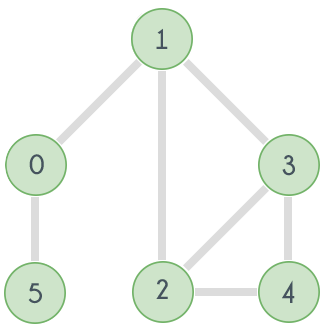
\includegraphics[width=\linewidth/6*2]{cutpoint.png}
\caption{Örneğin 0 düğümünü çıkardığımızda düğümler {${5}$} ve {${1, 2, 3, 4}$} olmak üzere iki gruba ayrılıyor. Aynı şekilde 1 düğümünü çıkardığımızda düğümler {${5, 0}$} ve {${2, 3, 4}$} olmak üzere iki gruba ayrılıyor. Bu nedenle 0 ve 1 düğümleri birer \textbf{articulation point}'dir. }
\label{fig:prime1}
\end{figure}
    
    \subsection{Articulation Point Bulma}
    Articulation point'leri bulmak için kullanacağımız Tarjan'ın algoritması:
    
\begin{itemize}
	\item Çizgeyi dfs order ile gez.
	\item Her düğüm için o düğümden ve alt ağacından yukarı çıkan kenarlardan minimum derinklikli düğüme gidenin derinliğini hesapla. Bu değere düğümün alt ağacından ulaşabileceğimiz minimum derinlik diyebiliriz. (Buna \textbf{low} değeri diyeceğiz.)
	\item Eğer root olmayan herhangi bir düğümün çocuklarından birinin \textbf{low} değeri şu anki düğümün derinliğinden büyük veya eşitse bu düğüm \textbf{articulation point}dir. Çünkü bu düğümün alt ağacındaki hiçbir \textbf{back edge}, şu anki düğümün üstünde bir düğüme çıkmamaktadır. Dolayısıyla bu düğümü çıkardığımızda bu düğümün alt ağacı ve ataları birbirinden ayrılır.
	\item Eger şu anki düğümümüz root(Dfs order'a başladığımız düğüm) ise, dfs ile gezerken birden fazla kez dallanmamız root'un \textbf{Articulation Point} olmasına sebep olur. Çünkü root'un bağlı olduğu birden fazla ayrık alt-çizgesi vardır.
\end{itemize}

Tarjanın algoritmasıyla çizgedeki articulation pointleri O(V + E) zaman karmaşıklığında bulabiliriz.

\cleardoublepage

    \begin{minted}[frame=lines,linenos,fontsize=\footnotesize]{c++}
int dfs(int node, int parent, int depth){
	int minDepth = depth, children = 0;
	dep[node] = depth;// dep dizisi her dugumun derinligini tutmaktadir.
	used[node] = true;
	for(auto it : g[node]){
		if(it == parent)
			continue;
		if(used[it]){
			minDepth = min(minDepth, dep[it]);
			continue;
		}
		int val = dfs(it, node, depth + 1);
		if(val >= depth and parent != -1)
			isCutPoint[node] = true;
		minDepth = min(minDepth, val);
		children++;
	}
	//Bu if yukarida belirttigimiz root olma durumunu kontrol ediyor.
	if(parent == -1 and children >= 2)
		isCutPoint[node] = true;
	return minDepth;
}
    \end{minted}
    
    
    \cleardoublepage
	
	
	\section{Strong Connectivity and Biconnectivity}
	
	\subsection{Strong Connectivity}
	 Bir düğümden hedef bir düğüme ulaşılabilmesi için, sonlu sayıda düğümden geçerek hedef düğüme varılması gerekmektedir.
	
	Yönsüz bir çizgede her düğümden diğer her düğüme ulaşılabiliyorsa bu çizgeye \textbf{connected} denir. Aynı konsept yönlü çizgelere uygulandığında bu sefer ismi \textbf{strongly connected} olmaktadır.
	
	Yani bir yönlü çizgenin \textbf{strongly connected} olması için her düğümden diğer bütün düğümlere ulaşılabilmesi gerekmektedir.
	\subsection{Biconnectivity}
	Yönsüz bir çizgede herhangi bir düğüm silindiğinde eğer geriye kalan çizge \textbf{connected} oluyorsa bu çizgeye \textbf{biconnected} denir. Başka bir deyişle çizgede \textbf{articulation point} yoksa bu çizge \textbf{biconnected} bir çizge olmaktadır.
\begin{figure}[H]
\centering
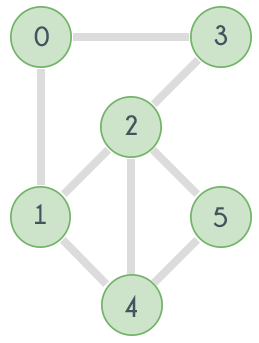
\includegraphics[width=\linewidth/3]{biconnectivity.png}
\caption{Biconnected bir graph örneği.}
\label{fig:prime1}
\end{figure}


	\cleardoublepage

    \section{Connected Components}
    \subsection{Strongly Connected Components}
   Bütün yönlü çizgeler \textbf{strongly connected} olan ayrık alt-çizgelere bölünebilir. İki alt-çizgenin ayrık olması için ortak kenar ve düğüm içermemesi gerekmektedir. Oluşan alt-çizgeleri tek bir düğüm olarak düşünüp yeni bir çizge oluşturursak, oluşan yeni çizge, içinde cycle olmayan yönlü bir çizge oluşturur.
\begin{figure}[H]
\centering
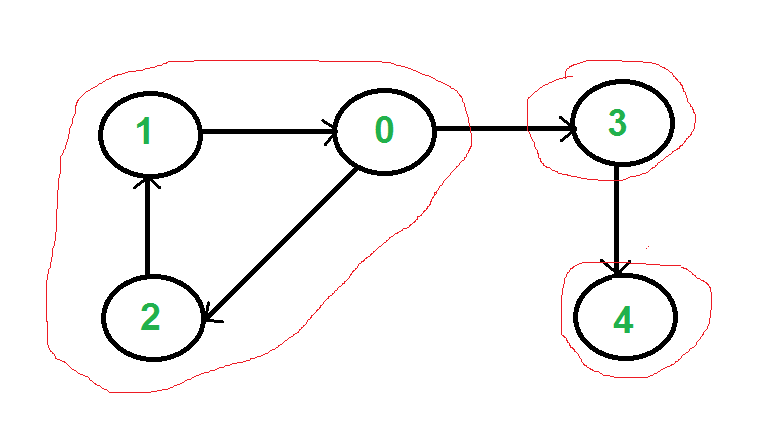
\includegraphics[width=\linewidth/2]{SCC.png}
\caption{Kırmızı ile işaretli olan alt-çizgeler \textbf{strongly connected component}lerdir.}
\label{fig:prime1}
\end{figure}

\begin{figure}[H]
\centering
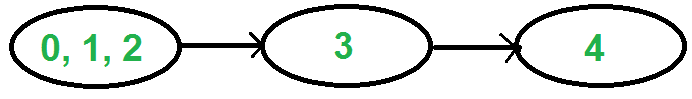
\includegraphics[width=\linewidth/2]{SCCGraph.png}
\caption{Oluşan yeni çizge içinde cycle olmayan yönlü bir çizge oluşturur.}
\label{fig:prime1}
\end{figure}

Strongly connected componentleri bulmak için kullanacağımız Tarjan'ın algoritması(Alternatif olarak Kosaraju Algoritması da bulunmaktadır fakat pratikte daha yavaş olduğundan ve anlamasının zor olmasından kaynaklı tarjanın algoritmasını ele alacağız):

\begin{itemize}
	\item Herhangi bir düğümden dfs order ile gezmeye başla ve uğradığı düğümleri bir stack(yığın)'a at. Her düğümün keşfedilme zamanını hesapla. (Keşfedilme zamanı, dfs order ile gezerken düğüme ilk geldiğimiz birim zamandır ve buna \textbf{index} diyeceğiz)
	\item Eğer bir düğüm stack'in içindeyse henüz herhangi bir strongly connected component'e ait değildir. Bunun sebebi ise strongly connected component bulduğumuz zaman stack'deki strongly connected componente ait olan düğümleri çıkarmamızdır.
	\item Her düğüm için o düğümden ve alt ağacından yukarı çıkan, herhangi bir strongly connected component'e ait olmayan düğümlere giden kenarlardan, minimum indexe sahip düğüme gidenin indexini hesapla. Bu değere düğümün alt ağacından ulaşabileceğimiz minimum derinlik diyebiliriz. (Buna \textbf{low} değeri diyeceğiz.)
	\item Eger bir düğümün low değeri kendi indexine eşit ise bu düğüm ve bu düğümün altındaki stack'deki tüm düğümler strongly connected component'dir. Bunun sebebi ise eğer bu düğüme \textbf{u} dersek; \textbf{u}'nun alt-ağacından kendisine gelen bir kenar mutlaka olmak zorundadır çünkü olmaması durumunda \textbf{u}'nun low değerinin kendi index'inden daha küçük bir değer olacağı barizdir.
	\item Strongly connected component bulunduğunda(bir önceki adımda nasıl bulunduğu açıklanmıştır) stack'den şuanki strongly connected componente ait tüm düğümleri çıkar.
\end{itemize}

Tarjanın algoritmasıyla çizgedeki strongly connected compenentleri O(V + E) zaman karmaşıklığında bulabiliriz.
    
      \begin{minted}[frame=lines,linenos,fontsize=\footnotesize]{c++}
void dfs(int node){
	low[node] = index[node] = ++curTime;
	// curTime her dugumun kesfedilme zamanini bulmamizi sagliyor.
	used[node] = true;

	st.push(node);
	inStack[node] = true;
    // Bir dugumun stackte olup olmadigini inStack dizisiyle tutmamiz gerekiyor.
	for(auto it : g[node]){
		if(!used[it]){
			dfs(it);
			low[node] = min(low[node], low[it]);
		}
		else if(inStack[it])
			low[node] = min(low[node], index[it]);
//Eger komsu dugum stack icindeyse o zaman bu edge back edge olabilir.
	}
	if(low[node] == index[node]){
		while(1){
			int x = st.top();
			st.pop();
			cout << x << " ";
			inStack[x] = false;
			if(x == node)
				break;
		}
		cout << endl;
	}
}

void scc() {
	for(int i = 0; i < n; i++)
		if(!used[i])
			dfs(i);
}
    \end{minted}
    \cleardoublepage
    
    \section{Cycle Finding}
    \subsection{Cycle bulma}
    
    \textbf{Cycle}: başladığı düğüme geri dönen, her düğümü en fazla bir defa gezen ve en az 2 düğüm içeren düğüm dizisidir.
    
    Bir çizgede cycle olup olmadığını bulmak için Dfs order kullanabiliriz.
    
    Eğer Dfs order ile gezerken back edge ile karşılaşırsak o zaman çizgede cycle vardır. Çünkü \textbf{back edge} üst ve alt ucundaki düğümü birbirine bağlayıp cycle oluşmasına sebep olmaktadır.

    Yönlü bir çizgede cycle bulmak için kullancağımız algoritma:
    
\begin{itemize}
    \item Çizgeyi dfs order ile gez.
	\item Bir düğüme geldiğinde o düğümü griye boya ve komşularını gezmeye başla.
	\item Eğer şu anki düğümün komşularından bir tanesi gri ise o zaman çizgede cycle vardır. Çünkü gri olan bir düğüm kesinlikle şu anki düğümün atalarındandır ve kendi atalarından bir düğüme giden bir kenarın back edge olduğu kesindir.
	\item Komşuları gezmeyi tamamladıktan sonra düğümü siyaha boya.
\end{itemize}


    
    \begin{minted}[frame=lines,linenos,fontsize=\footnotesize]{c++}
bool dfs(int node){
    //color dizizi her nodeun rengini tutuyor.
    //Eger color degeri 0 ise beyaz, 1 ise gri, 2 ise siyah rengini temsil ediyor.
	color[node] = 1;
	for(int i = 0; i < g[node].size(); i++){
		int child = g[node][i];
		if(color[child] == 1)
			return true;
		if(!color[child])
			if(dfs(child))
				return true;
	}
	color[node] = 2;
	return false;
}

    \end{minted}


    \cleardoublepage

    \section{Max Flow}
    \subsection{Flow Network}
    \textbf{Flow network} bir adet \textbf{kaynak} ve bir adet \textbf{hedef} içeren özel bir yönlü çizge çeşididir.


    Flow network çizgesinde her kenarın bir kapasitesi vardır. Bu kapasiteler bu kenarden geçebilecek flow(akış) miktarını belirtmektedir.
    
    \begin{figure}[H]
\centering
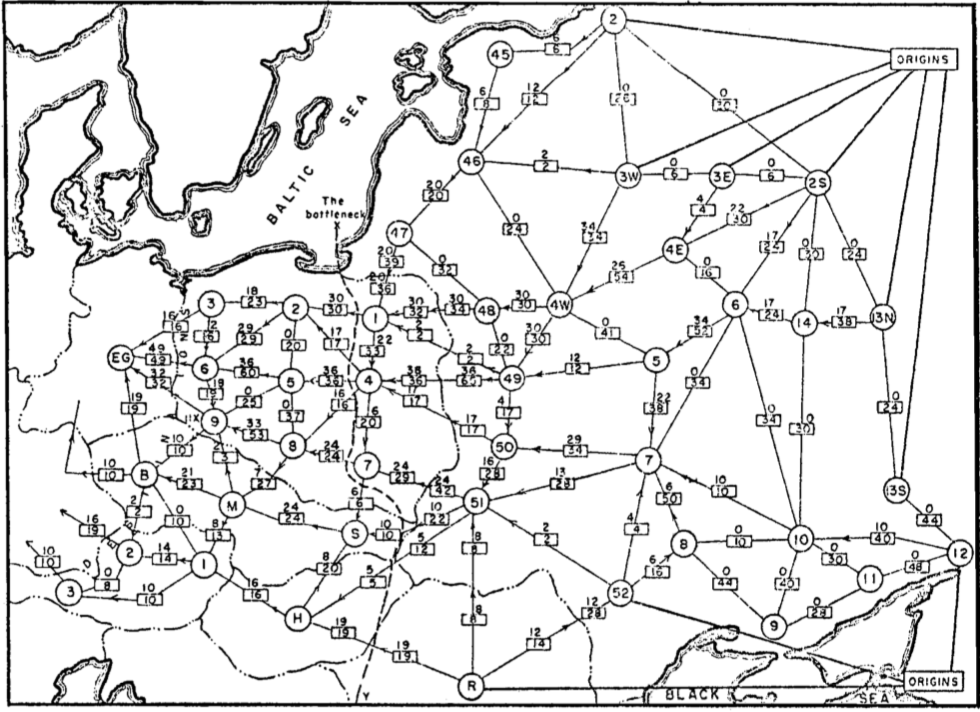
\includegraphics[width=\linewidth/3*2]{ilkflow.png}
\caption{Tarihteki ilk flow network örneklerinden biri.}
\label{fig:prime1}
\end{figure}

    
    \subsection{Maximum Flow}
    
    Maximum flow belirli bir flow networkünde kaynaktan hedefe devamlı bir akış varken birim zamanda hedefe ulaşabilecek maximum akış miktarını hesaplayan algoritmadır.
    
    Maximum Flow problemini çözmeye yarayan bir çok algoritma vardır. Bunlardan popüler olanların zaman karmaşıklıkları:
     \begin{itemize}
    \item Ford-Fulkerson algoritması : $O(E * flowSayisi)$
    \item Edmonds–Karp algoritması : $O(V * E^2)$
    \item Dinic algoritması : $O(E * V^2)$
    \end{itemize}

    \subsection{Ford Fulkerson}
    Ford Fulkerson'un maximum flow algoritmasının adımları şöyledir:
    \begin{itemize}
    \item Kaynaktan hedefe bir yol bul.
    \item Bulduğumuz yoldaki minimum kapasiteli kenar bu yoldan geçebilecek flowa eşittir.
    
    \item Yoldaki kenarların kapasitelerini bulduğumuz flow(adım 2 de bulduğumuz minimum kapasite) kadar eksilt ve kullandığımız kenarların tersini bulduğumuz flow kadar kapasiteli olacak şekilde çizgeye ekle.
    
    \item Kaynaktan hedefe yol kalmayana kadar devam et.
    \end{itemize}


    Peki bu neden çalışıyor?

    Örneğin \textbf{u}'dan \textbf{v}'ye olan kenarı içeren \textbf{x} büyüklüğünde bir flow bulduğumuzu varsayalım.
    
    Bulduğumuz yol $a \rightarrow ... \rightarrow u \rightarrow v \rightarrow ... \rightarrow b$ olsun.
    
    Çizgemize \textbf{v}'den \textbf{u}'ya \textbf{x} kapasitelli yeni bir kenar ekleyeceğiz fakat bulduğumuz bu kenar orjinal çizgemizde bulunmuyor.

    Ters kenarları ekledikten sonra bulduğumuz yeni yol da $c \rightarrow ... \rightarrow v \rightarrow u \rightarrow ... \rightarrow d$ olsun ve bulunan flow da \textbf{y} olsun.

    $y \leq x$  olduğu barizdir.

    $a \rightarrow ... \rightarrow u \rightarrow ... \rightarrow d$ yolunu izleyen \textbf{y} büyüklüğünde bir flow,

    $c \rightarrow ... \rightarrow u \rightarrow ... \rightarrow b$ yolunu izleyen \textbf{y} büyüklüğünde bir flow,

    $a \rightarrow ... \rightarrow u \rightarrow v \rightarrow ... \rightarrow d$ yolunu izleyen  \textbf{x - y} büyüklüğünde bir flow olacak şekilde 3 farklı geçerli flow şeklinde gösterebiliriz.

    Ford Fulkersenin genel çalışma karmaşıklığı $O(E * flowSayisi)$ çünkü en kötü durumda her yol bulduğunda flowu 1 arttırır. Her yol bulma işlemi de kenar sayısı kadar olduğuna göre karmaşıklık $O(E * flowSayisi)$ olur.
    Fakat Ford Fulkersen algoritmasını kodlarken BFS kullanırsak o zaman karmaşıklık; her kenar için o kenarı minimum kabul eden flowların sürekli artacak olmasından dolayı $O(V*E^2)$ oluyor. Bu implementasyona Edmond-Karp Algoritması deniyor.
    \cleardoublepage
    
\begin{figure}[H]
\centering
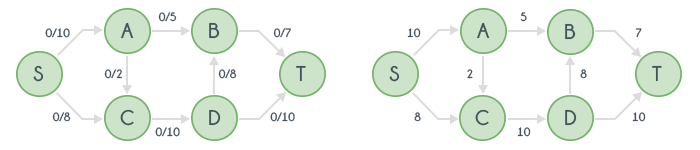
\includegraphics[width=\linewidth/4*3]{flow1.png}
\caption{Soldaki figür her kenardan ne kadar flow geçtiğini gösteriyor. Sağdaki ise çizgenin şu anki halini gösteriyor.}
\label{fig:prime1}
\end{figure}

\begin{figure}[H]
\centering
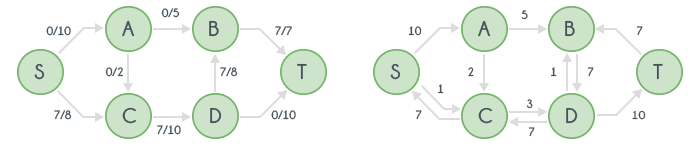
\includegraphics[width=\linewidth/4*3]{flow2.png}
\caption{Flow = 7}
\label{fig:prime1}
\end{figure}

\begin{figure}[H]
\centering
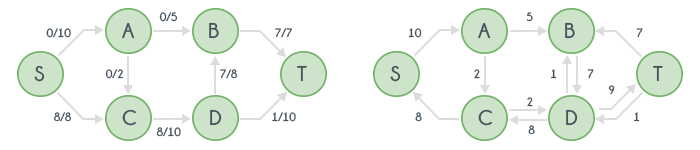
\includegraphics[width=\linewidth/4*3]{flow3.png}
\caption{Flow = 8}
\label{fig:prime1}
\end{figure}

\begin{figure}[H]
\centering
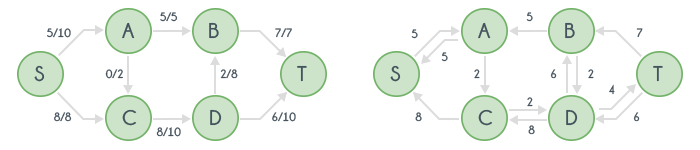
\includegraphics[width=\linewidth/4*3]{flow4.png}
\caption{Flow = 13}
\label{fig:prime1}
\end{figure}

\begin{figure}[H]
\centering
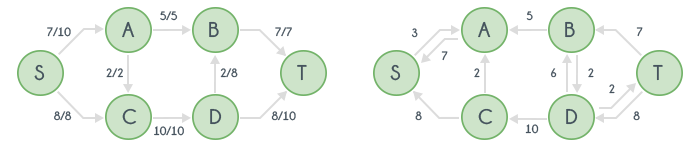
\includegraphics[width=\linewidth/4*3]{flow5.png}
\caption{Flow = 15}
\label{fig:prime1}
\end{figure}
    
    \cleardoublepage
    \begin{minted}[frame=lines,linenos,fontsize=\footnotesize]{c++}
//c matrisi her kenarin kapasitesini tutuyor.
//g komsuluk listesi ise cizgeyi gezmemizi sagliyor.
bool bfs(){
	vector < bool > visited(n, false);
	queue < int > q;
	q.push(source);
	visited[source] = true;
	while(!q.empty()){
		int node = q.front();
		q.pop();
		if(node == sink)
			break;
		for(int i = 0; i < g[node].size(); i++){
			int child = g[node][i];
			if(c[node][child] <= 0 or visited[child])
				continue;
			visited[child] = true;
			parent[child] = node;
			q.push(child);
		}
	}
	return visited[sink];
}
int max_flow() {
    while(bfs()){
	int curFlow = -1, node = sink;
	while(node != source){
	//curFlow su anki yoldaki minimum kapasite yani buldugumuz flowdur.
		int len = c[parent[node]][node];
		if(curFlow == -1)
			curFlow = len;
		else
			curFlow = min(curFlow, len);
		node = parent[node];
	}
	flow += curFlow;
	node = sink;
	while(node != source){
		c[parent[node]][node] -= curFlow;
		//Buldugumuz yoldan buldugmuz flowu eksiltiyoruz.
		c[node][parent[node]] += curFlow;//Kenarlarin tersini ekliyoruz.
		node = parent[node];
        }
    }
    return flow;
}
    \end{minted}
    
    \cleardoublepage
    
\newpage
\begin{thebibliography}{9}
\bibitem{1}
\href{https://cp-algorithms.com/graph/bridge-searching.html}{Finding bridges in a graph in O(N+M). CP-Algorithms.}
\bibitem{2}
\href{https://www.geeksforgeeks.org/articulation-points-or-cut-vertices-in-a-graph/}{Articulation Points (or Cut Vertices) in a Graph. Geeksforgeeks website.}
\bibitem{3}
\href{https://www.geeksforgeeks.org/tree-back-edge-and-cross-edges-in-dfs-of-graph/}{Tree, Back, edge and Cross edges in DFS of Graph. Geeksforgeeks website.} 
\bibitem{4}
\href{https://en.wikipedia.org/wiki/Cycle_detection}{Cycle detection. Wikipedia, the free online encyclopedia.}
\bibitem{5}
\href{https://www.hackerearth.com/practice/algorithms/graphs/maximum-flow/tutorial/}{Maximum flow from hackerearth.}
\bibitem{6}
\href{https://www.geeksforgeeks.org/ford-fulkerson-algorithm-for-maximum-flow-problem/}{Ford-Fulkerson Algorithm for Maximum Flow Problem. Geeksforgeeks website.}
\bibitem{7}
\href{https://www.geeksforgeeks.org/tarjan-algorithm-find-strongly-connected-components/}{Tarjan’s Algorithm to find Strongly Connected Components. Geeksforgeeks website.}
\bibitem{8}
\href{https://www.hackerearth.com/practice/algorithms/graphs/strongly-connected-components/tutorial/}{Strongly Connected Components. Hackerearth website.}
\bibitem{9}
\href{https://www.hackerearth.com/practice/algorithms/graphs/articulation-points-and-bridges/tutorial/}{Articulation Points and Bridges. Hackerearth website.}
\bibitem{10}
\href{https://en.wikipedia.org/wiki/Connected_component_(graph_theory)}{Connected component (graph theory). Wikipedia, the free online encyclopedia.}
\bibitem{11}
\href{https://en.wikipedia.org/wiki/Tarjan\%27s_strongly_connected_components_algorithm}{Tarjan's strongly connected components algorithm. Wikipedia, the free online encyclopedia.}
\bibitem{12}
\href{https://en.wikipedia.org/wiki/Flow_network}{Flow Network. Wikipedia, the free online encyclopedia.}
\bibitem{13}
\href{https://link.springer.com/article/10.1007\%2Fs101070100259}{On the history of the transportation and maximum flow problems}
\bibitem{14}
\href{https://en.wikipedia.org/wiki/Edmonds–Karp_algorithm}{Edmonds–Karp algorithm. Wikipedia, the free online encyclopedia.}
\bibitem{15}
\href{https://en.wikipedia.org/wiki/Biconnected_graph}{Biconnected graph. Wikipedia, the free online encyclopedia.}

\end{thebibliography}        
\end{document}
     

\end{document}